\chapter{OshiFitの設計と実装}
本章では，第3章で導いた設計指針D1〜D4に基づいて構築したシステムOshiFitについて述べる．まずシステムの全体像と利用の流れを示し，続いて質問紙，得点の算出，群の振り分け，提案の選択，プランA・Bの見込み，アバターの生成，週ごとの振り返り，データ管理，安全への配慮，実装の順に述べる．

\section{システムの概要}
OshiFitは，利用者の性格特性と推し活の状況を質問紙で把握し，推し活の状態を6つの軸で可視化したうえで，本人に合った推し活の整え方（プラン）を提案するWebアプリケーションである．利用者は，プランを取り入れなかった場合（プランA：現在のままの推し活）と取り入れた場合（プランB：最適化された推し活）の6週間後の見込みを，本人に似たアバターと数値で見比べ，どちらにするかを自分で選ぶ．選んだ後は，6週間にわたって週1回の振り返りを行い，プランの実行状況と推し疲れの変化を記録する．

OshiFitの特徴は次の4点である．
\begin{enumerate}
\item 一律に減らす助言をせず，「今のまま」も常に選べる（D1）．
\item 本人の行動と負担の状況に合わせてプランを選び，性格は優先順位の調整に用いる（D2）．
\item 幸福度と推し疲れを6つの軸で同時に示し，算出式も開示する（D3，D4）．
\item 見込みを80\%の幅とともに示し，差が小さいときは「ほぼ同じ」と伝える（D4）．
\end{enumerate}

\section{利用の流れ}
表\ref{tab:flow}に，OshiFitの利用の流れを示す．

\begin{table}[t]
\centering
\jetcaption{OshiFitの利用の流れ}{User flow of OshiFit}
\label{tab:flow}
\small
\begin{tabular}{@{}p{0.17\linewidth}p{0.37\linewidth}p{0.38\linewidth}@{}}
\toprule
段階 & 利用者が行うこと & システムが行うこと \\
\midrule
開始時（約10分） & 説明を読んで同意し，67項目の質問紙に回答する．写真または部品を選んでアバターを作る & 6軸の得点，推し疲れ（総合），性格（ビッグファイブ），推し活の傾向を計算して表示する．算出根拠も表示する \\
振り分け & 結果を見る & 6軸のうち5軸以上が60点以上，かつWHO-5の素点が13点以上なら群A（今のままで順調）とする．それ以外はプランA・Bを表示する \\
選択 & プランAとプランBを見比べ，どちらにするかを選ぶ & プランBを選んだら群B，プランAを選んだら群Cとして記録する \\
6週間 & 群B・C：週1回以上，振り返りに答える（約2分）．群A：利用は不要 & プランの実行状況，推し疲れ4項目，推し活中の幸福感，変化の自己評価を記録する \\
6週目 & 全員が終了調査（WHO-5を含む）に答える．群B・Cは使いやすさ等にも答える & 開始時と6週目のレーダーチャートを重ねて表示する \\
\bottomrule
\end{tabular}
\end{table}

\section{質問紙}
\subsection{構成}
OshiFitの質問紙は67項目からなる（表\ref{tab:questionnaire}）．第3章の調査で用いた調査票を基に，次の点を修正した．
\begin{enumerate}
\item \textbf{頻度の聞き方}：回数ではなく，「自分の推し活全体の中で，その活動がどのくらいの割合を占めているか」を5段階（まったくしない〜中心）で尋ねる形にした．推し活の量は人によって大きく異なるため，絶対的な回数よりも本人の中での相対的な比重の方が，提案の手がかりとして解釈しやすいと考えたためである．
\item \textbf{選択肢の向きの統一}：第3章の調査では回答の向きの取り違えが起きたため，すべての項目で「数字が大きいほど多い・強い」向きにそろえた．
\item \textbf{金額の聞き方}：収入に対する予算の割合は欠損が多かったため，1か月あたりの金額の区分で尋ねる形にした．
\item \textbf{TIPI-J}：第3章と同じ文言を5件法で用いた\cite{oshio2012}．
\item \textbf{WHO-5の追加}：開始時と6週目の精神的健康を比較するため，WHO-5（5項目）\cite{topp2015,inagaki2013}を追加した．
\item \textbf{主たる推しの定義}：「いま最も時間を使っている推しを1人・1組」と明記した．
\item \textbf{注意確認項目}：データの品質確認のため残した．
\end{enumerate}

\begin{table}[t]
\centering
\jetcaption{OshiFitの質問紙の構成（全67項目）}{Structure of the OshiFit questionnaire (67 items)}
\label{tab:questionnaire}
\small
\begin{tabular}{@{}p{0.3\linewidth}p{0.38\linewidth}p{0.22\linewidth}@{}}
\toprule
区分 & 項目 & 回答形式 \\
\midrule
基本情報 & Q1〜Q6（年齢，性別，職業，推しのジャンル，応援期間，1か月の金額の区分） & 選択 \\
性格（TIPI-J） & Q7〜Q16 & 5件法 \\
推し活の内容（割合） & Q17〜Q28（音楽，動画，ライブ，CD，グッズ，テレビ・ラジオ，雑誌，SNSのチェック，SNSでの発信，聖地巡礼，ファンクラブ，コラボカフェ） & 5段階 \\
気持ちと生活の変化 & Q29〜Q54（充実，生活管理，能力，交流，負担．注意確認Q42を含む） & 7件法 \\
推し活をしたくなるとき & Q55〜Q61（逃避，孤独，ご褒美，回復，SNSの影響，習慣，気分の高揚） & 7件法 \\
WHO-5 & W1〜W5（最近2週間） & 6件法（0〜5） \\
自由記述 & Q62（任意） & 記述 \\
\bottomrule
\end{tabular}
\end{table}

全項目は付録Aに示す．

\subsection{件法の選択}
気持ちと生活の変化，推し活をしたくなるときの項目は7件法とした．これらは推し活の便益と負担の微妙な程度の違いを捉える必要があり，また第3章の調査との比較のためである．一方，推し活の内容は「割合」を尋ねるため，「まったくしない」「ごく一部」「一部」「大きな部分」「中心」の5段階とした．性格は第3章と同じく5件法とした．件法は項目の性質に応じて選んでおり，すべてを統一することはしていない．

\section{6軸の得点}
OshiFitは，質問紙の回答から推し活の状態を6つの軸で0〜100点に換算し，レーダーチャートで示す（表\ref{tab:axes}）．すべての軸は外側ほど良好になるようにそろえた．負担を表す軸（睡眠・生活，お金，義務感・人間関係，SNS・比較）は，負担の項目の平均を逆にして，点数が高いほど負担が少ないことを表す．画面には，各軸の算出式と，その計算に使った本人の回答も表示する（D4）．

\begin{table}[t]
\centering
\jetcaption{6軸の得点と推し疲れ（総合）の算出式}{Formulas for the six axes and overall burnout}
\label{tab:axes}
\small
\begin{tabular}{@{}p{0.22\linewidth}p{0.2\linewidth}p{0.48\linewidth}@{}}
\toprule
軸 & 使用項目 & 算出式 \\
\midrule
幸福度 & W1〜W5 & WHO-5の合計（0〜25）$\times4$ \\
推し活の充実 & Q29〜Q34，Q39 & （7項目の平均$-1$）$\div6\times100$ \\
睡眠・生活 & Q44，Q50 & $100-$（2項目の平均$-1$）$\div6\times100$ \\
お金 & Q45，Q46 & $100-$（2項目の平均$-1$）$\div6\times100$ \\
義務感・人間関係 & Q47，Q49 & $100-$（2項目の平均$-1$）$\div6\times100$ \\
SNS・比較 & Q48，Q51 & $100-$（2項目の平均$-1$）$\div6\times100$ \\
\midrule
推し疲れ（総合） & Q44〜Q51 & （8項目の平均$-1$）$\div6\times100$（高いほど推し疲れ） \\
\bottomrule
\end{tabular}
\end{table}

\section{群の振り分け}
6軸のうち5軸以上（約8割）が60点以上，かつWHO-5の素点が13点以上の利用者には，「今の推し活は順調です」と伝え，プランは提示しない（群A）．60点は7件法で「どちらともいえない」より良い側に入る点であり，WHO-5の13点は精神的健康が良好であるとされる目安である\cite{topp2015}．すでに良好な人に変更を勧めないことは，設計指針D1に基づく．

\section{プランの選択}
群Aに当てはまらない利用者には，11種類のプランの中から3案を提示する（表\ref{tab:plans}）．各プランは，6軸のうちいずれか1つの改善を狙うものであり，第3章の結果（便益と負担が同じ行動から生じること，SNSを減らしたい人が一定数いること）に基づき，活動そのものをやめるのではなく，関わり方を整える内容とした．

\begin{table}[t]
\centering
\jetcaption{OshiFitの11種類のプラン}{Eleven plans in OshiFit}
\label{tab:plans}
\small
\begin{tabular}{@{}p{0.15\linewidth}p{0.42\linewidth}p{0.17\linewidth}p{0.14\linewidth}@{}}
\toprule
対象の軸 & プラン & 想定改善量（点） & 優先する性格 \\
\midrule
睡眠・生活 & SNSは23時まで．そのあとはお休みモード & 16 & -- \\
睡眠・生活 & リアタイは週2回まで，ほかはアーカイブで & 12 & 誠実性 \\
お金 & 今月のグッズ予算を先に決める & 16 & 誠実性 \\
お金 & 欲しいグッズは1日おいてから決める & 12 & 神経症傾向 \\
義務感 & 今週追うものを3つに絞る & 15 & -- \\
義務感 & 「行かない回」を1つ決めておく & 12 & 誠実性 \\
SNS・比較 & 比べてしまう言葉をミュートする & 15 & 神経症傾向 \\
SNS・比較 & SNSを見るのは1日2回・各15分まで & 12 & 外向性（低） \\
推し活の充実 & 友達と同時視聴の日をつくる & 12 & 外向性 \\
推し活の充実 & 感想メモや創作で推しを残す & 12 & 開放性 \\
推し活の充実 & 寝る前15分は推しの曲だけの時間 & 10 & 協調性 \\
\bottomrule
\end{tabular}
\end{table}

プランは次の手順で選ぶ．まず，6軸を点数の低い順に並べ，点数の低い軸に対応するプランほど優先する．同じ程度の優先度のプランの間では，利用者の性格の傾向に合うプランを優先する（例：誠実性が高い人には予算を先に決めるプラン，神経症傾向が高い人には比較の言葉をミュートするプラン）．3案の対象の軸が重ならないようにし，利用者が異なる方向の提案を比較できるようにする．各プランには，具体的な実行方法（例：「通知を23時にオフにし，翌朝まとめて見る」）と，選ばれた理由（例：「睡眠・生活が33点」）を表示する．これは，推薦の理由を示すことで利用者が提案を自ら評価して選べるようにするためである\cite{tintarev2007}．また，小さく実行しやすい行動を具体的な手順とともに示すことは，行動変容の理論\cite{fogg2009}とも整合する．

プランの選択は決定的な規則で行い，機械学習による学習は行わない．これは，検証実験の期間中に参加者ごとに提案の仕組みが変わらないようにし，提案の根拠を利用者と研究者の双方が確認できるようにするためである．

\section{プランAとプランBの見込み}
\subsection{見込みの算出}
プランAは，現在の回答から計算した6軸の得点をそのまま用いる．プランBは，選んだプランが対象の軸を一定の点数（v1.0ではプランごとに10〜16点，表\ref{tab:plans}）改善し，幸福度がその4分の1だけ上がると仮定して算出する．この想定改善量は，第3章の結果（推し活の頻度を1段階変えたときの予測値の変化）と，プランの実行しやすさを踏まえて設定した暫定的な値であり，検証実験の期間中はv1.0に固定する．

\subsection{不確かさの表示}
第3章の結果から，個人の予測には大きな誤差が伴うことが分かった．そこでOshiFitでは，各軸に$\pm15$点，幸福度に$\pm12$点の幅を80\%の幅の目安として表示する（D4）．幅は，前研究の予測誤差に基づいて設定した．予測の不確かさを可視化することで利用者がより適切な判断を行えることは，Kayら\cite{kay2016}の研究でも示されている．また，プランAとプランBの差が5点未満のときは「ほぼ同じ」と表示し，わずかな差を過大に受け取らないようにする．画面には「この見込みは将来を決めるものではなく，診断でもありません．今のままを選ぶこともできます」と明記する．

図\ref{fig:twofutures}に，2つの未来の表示の例を示す．

\begin{figure}[t]
\centering
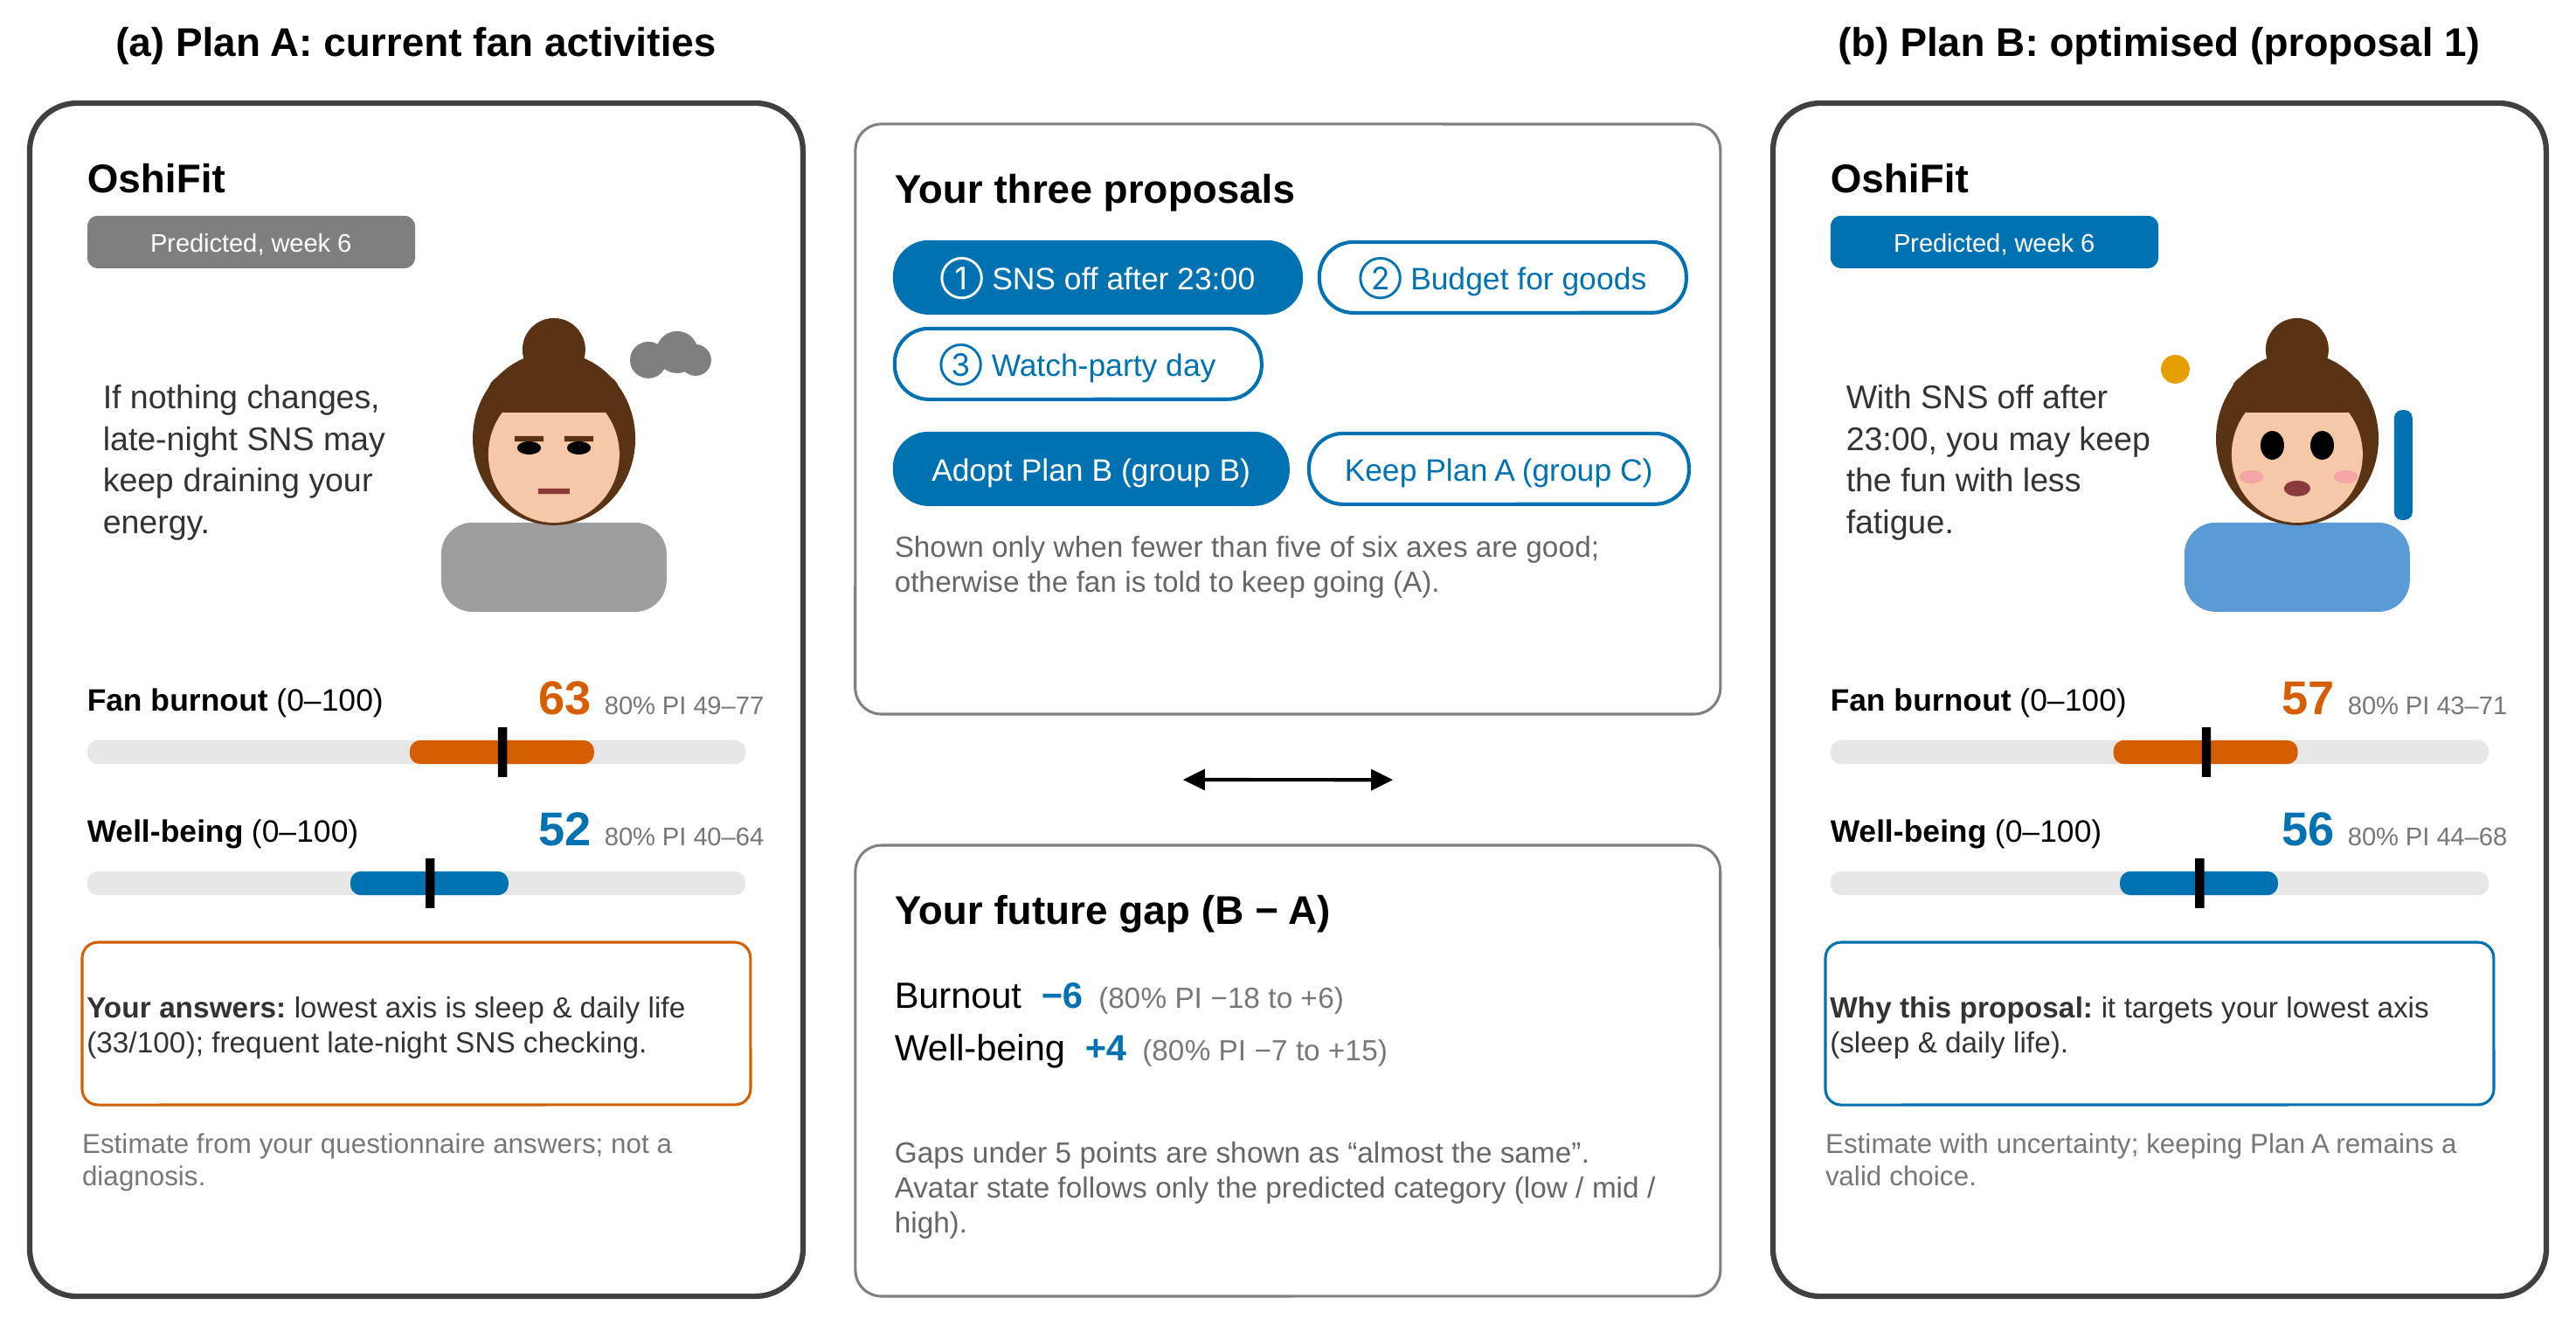
\includegraphics[width=\linewidth]{figures/fig2_twofutures_ppt.png}
\jecaption{OshiFitの「2つの未来」の表示（架空の利用者の例）．プランA（現在のままの推し活）とプランB（最適化された推し活）の6週間後の推し疲れと幸福度の見込みを80\%の幅とともに示す}{OshiFit's two-futures display (illustrative user)}
\label{fig:twofutures}
\end{figure}

\section{アバターの生成}
OshiFitでは，本人に似た2Dアバターで状態を表す．これは，本人に似た姿で将来の状態を見せることが行動のきっかけになりうるという，プロテウス効果や将来の自己に関する研究\cite{yee2007,fox2009,hershfield2011}に基づく．

アバターは，利用者が撮影または選択した顔写真から，端末の中で作成する．Googleが提供するMediaPipe\cite{lugaresi2019}の顔の特徴点検出を端末内で動かし，顔の幅と高さの比（顔の形），目の開き，眉の傾き，口の幅を測ってアバターの部品に反映する．肌と髪の色も写真から読み取る．写真と特徴点は端末の外に送らず，読み取り後すぐに破棄し，保存するのは部品の番号だけである．写真を使いたくない利用者は，部品を自分で選んでアバターを作ることもできる．

アバターの表情は，6軸の平均点の区分だけで決まる．平均が50点未満なら疲れ気味，50〜64点ならふつう，65点以上なら元気な表情とする．数値の区分に対応させ，大げさな表現は行わない．プランAとプランBのアバターは，それぞれの見込みの区分に応じた表情で並べて表示する．

\section{週ごとの振り返り}
群Bと群Cの利用者は，6週間にわたり週1回以上，振り返りに回答する（約2分）．振り返りでは，(1)プランを実行したか（行った・一部行った・行わなかった），(2)推し疲れの4項目，(3)推し活中の幸福感，(4)ストレスと幸福感の変化の自己評価を尋ねる．\todo{要確認：振り返り項目の最終版の文言（付録C）}

群Bで，プランを「行った」または「一部行った」週のうち，ストレスが「減った」かつ幸福感が「下がっていない」週は，正解データとしてアプリ内で自動的に印を付ける．この正解データは，検証実験の終了後にプランの想定改善量を更新するために用いる（5.7.6節）．

連絡先を集めない代わりに，毎週の振り返りと6週目の調査の日を，端末内で作成したカレンダー用ファイル（.ics）でカレンダーに追加できるようにした．

\section{データ管理と開発者ページ}
研究データは，Googleのクラウドサービス Firebase で一元管理する．データベース（Cloud Firestore）は東京リージョン（asia-northeast1）に置き，利用者は匿名認証で識別する．氏名や連絡先などの個人を特定できる情報は収集しない．利用者のデータは参加ID（匿名）ごとに保存し，セキュリティルールにより本人の記録だけを読み書きできるようにした．

研究者が全データを確認するための開発者ページ（admin.html）を用意し，閲覧できるのは本人（筆者）と指導教員のGoogleアカウントだけとした．開発者ページでは，参加者ごとの群，開始時の得点，週ごとの振り返り，6週目の結果を一覧でき，分析用にCSV形式で書き出せる．

\section{安全と参加者の負担への配慮}
推し活という本人にとって大切な趣味を扱うため，次の配慮を行った．
\begin{enumerate}
\item \textbf{相談先の表示}：開始時または6週目のWHO-5の素点が7点以下のとき，また週の振り返りで推し疲れ4項目の平均が6以上の週が2週続いたとき，相談先（学生相談室，厚生労働省「まもろうよ こころ」）を表示し，振り返りを休んでよいことを伝える．
\item \textbf{選択の尊重}：プランAを選ぶことも正当な選択として扱い，どちらを選んでも同じように振り返りを依頼する．
\item \textbf{参加の取りやめ}：マイページに参加ID（匿名）と「参加をやめる（記録を削除）」を表示し，押すとサーバー上と端末内の記録を削除する．
\item \textbf{写真の扱い}：写真と顔の特徴点は端末の外に送らず，保存しない．
\end{enumerate}

\section{実装}
OshiFitは，スマートフォンのブラウザで動作するWebアプリケーションとして実装した．画面はHTML，CSS，JavaScriptで作成し，Firebase Hosting で公開した．質問紙の項目と得点の算出規則はJSON形式の設定ファイルにまとめ，画面に表示する算出式と実際の計算が一致するようにした．アバターの生成にはMediaPipe Face Landmarker\cite{lugaresi2019}のWeb版を用いた．利用画面は，ホーム，分析，未来，マイページの4つのタブで構成し，質問紙への回答が終わって群が決まるまでは分析・未来のタブを表示しないようにした．また，一度選んだ群は変更できないようにした．

図\ref{fig:screens}に，OshiFitの主な画面を示す．

\begin{figure}[t]
\centering
\placeholderfig{70mm}{【要差し替え】OshiFitの画面のスクリーンショット（左から：質問紙，分析（6軸のレーダーチャートと算出根拠），未来（プランA・B），振り返り）\\ 公開版 https://oshifit-study.web.app から撮影して挿入する}
\jecaption{OshiFitの主な画面}{Main screens of OshiFit}
\label{fig:screens}
\end{figure}

本章では，OshiFitの設計と実装について述べた．第5章では，OshiFitの有用性を検証するために行う6週間の検証実験について述べる．
